\begin{figure}[H]
    \centering
    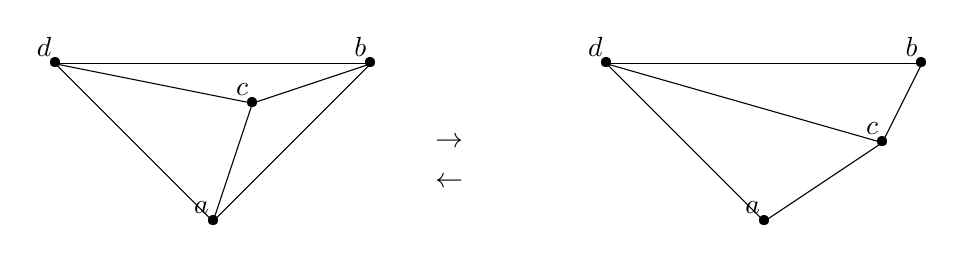
\begin{tikzpicture}
        \node[label={[label distance = -3mm]160:$a$}] at (0, 1) {\textbullet};
        \node[label={[label distance = -3mm]160:$b$}] at (2.0, 3.0) {\textbullet};
        \node[label={[label distance = -3mm]160:$c$}] at (0.5, 2.5) {\textbullet};
        \node[label={[label distance = -3mm]160:$d$}] at (-2.0, 3) {\textbullet};
        \draw (0, 1) -- (2.0, 3.0);
        \draw (0, 1) -- (0.5, 2.5);
        \draw (0.5, 2.5) -- (2.0, 3.0);
        \draw (0, 1) -- (-2.0, 3);
        \draw (-2.0, 3) -- (0.5, 2.5);
        \draw (-2.0, 3) -- (2.0, 3.0);

        \node at (3, 2.00) {$\rightarrow$};
        \node at (3, 1.5) {$\leftarrow$};

        \begin{scope}
            [shift={(7, 0)}]
            \node[label={[label distance = -3mm]160:$a$}] at (0, 1) {\textbullet};
            \node[label={[label distance = -3mm]160:$c$}] at (1.5, 2) {\textbullet};
            \node[label={[label distance = -3mm]160:$b$}] at (2.0, 3.0) {\textbullet};
            \node[label={[label distance = -3mm]160:$d$}] at (-2.0, 3) {\textbullet};
            \draw (0, 1) -- (1.5, 2);
            \draw (-2.0, 3) -- (1.5, 2);
            \draw (2.0, 3.0) -- (1.5, 2);
            \draw (0, 1) -- (-2.0, 3);
            \draw (-2.0, 3) -- (2.0, 3.0);
        \end{scope}
    \end{tikzpicture}
    \caption[Exemplo de evento \textsc{left}]{Exemplo de evento \textsc{left}.
    O ponto $c$ sai do fecho convexo, e por isso um triângulo é removido da triângulação.
    A Figura também pode ser vista da direita para à esquerda.}
    \label{fig:delaunay:left}
\end{figure}